% Manual and tutorial of OscTutorialPlugin (made from the AAT2 manual template, see docs/HowToDoc.md)
% Build (in docs/manual):  pdflatex ManualOscTutorialPlugin.tex   (twice, for the references)
% The PDF is copied into the release zips by the GitHub workflow.
% Figures: images/*.png, made with OscTutorialPlugin_Tester snapshot (see planning.md); measurements:
% tools/analysis/measure_models.py
\documentclass[11pt]{article}
\usepackage[utf8]{inputenc}
\usepackage[T1]{fontenc}
\usepackage{lmodern}
\usepackage[top=2cm, bottom=2cm, left=2.2cm, right=2.2cm]{geometry}
\usepackage{graphicx}
\usepackage{amsmath}
\usepackage{booktabs}
\usepackage{xcolor}
\usepackage{hyperref}
\hypersetup{colorlinks=true, linkcolor=red, urlcolor=red, citecolor=red, pdftitle={OscTutorialPlugin Documentation}}

% ---- change these ------------------------------------------------------------
\newcommand{\pluginversion}{1.0.1}   % the version in CMakeLists.txt
\newcommand{\pluginauthor}{Joerg Bitzer}
\newcommand{\sourceurl}{https://github.com/JoergBitzer/OscTutorialPlugin}
% -------------------------------------------------------------------------------

% two figures side by side: oscilloscope and spectrum of one model
\newcommand{\modelfigures}[2]{%
\begin{center}
\includegraphics[width=0.49\textwidth]{images/scope_#1.png}\hfill
\includegraphics[width=0.49\textwidth]{images/spectrum_#1.png}\\[-1ex]
{\small #2: sawtooth at C7 (2093\,Hz, 22.9 samples per period, 48\,kHz). Left: oscilloscope, right: spectrum.}
\end{center}}

\title{OscTutorialPlugin\\[1ex]\large Manual and tutorial: nine ways to make a sawtooth}
\author{\pluginauthor, Jade Hochschule Oldenburg\\License of this document: CC-BY 4.0}
\date{\today, for OscTutorialPlugin \pluginversion}

\begin{document}
\maketitle

\tableofcontents

\section{Introduction}
OscTutorialPlugin is a deliberately small synthesizer for teaching: one oscillator, one ADSR envelope,
monophonic. Its point is the \emph{oscillator model}: the same four waveforms (sine, triangle,
rectangle, sawtooth) can be made in nine different ways, from the naive one that every beginner
writes first, to band-limited tables, polynomial corrections and oversampling. You can switch
between them while a note sounds, and you can \emph{hear} the difference, \emph{see} it on the
built-in oscilloscope and spectrum and \emph{measure} it (section~\ref{sec:measure}).

(Until version 1.0.0 the plug-in was called VerySimpleSynth.)

Section~\ref{sec:tutorial} is a tutorial: why the naive oscillator aliases, how each method fights
that, and what it costs. Section~\ref{sec:exercises} has exercises for a lab session.

\textbf{Warning:} aliasing at high notes can be harsh and loud. Start with a low output level.

\section{Installation}
The downloaded file is a zip file. It contains the plug-in (.vst3; on macOS also the AU,
.component), the Standalone application, a ReadMeFirst.txt, the licence files and this manual.
Copy the plug-in to the right place and let your DAW rescan its plug-ins.

\begin{verbatim}
Windows (VST3):  C:\Program Files\Common Files\VST3
Mac (VST3):      /Users/yourUSERNAME/Library/Audio/Plug-Ins/VST3
Mac (AU):        /Users/yourUSERNAME/Library/Audio/Plug-Ins/Components
Linux (VST3):    /home/yourUSERNAME/.vst3
\end{verbatim}

The Standalone application needs no DAW: choose the audio and MIDI devices in its Options menu and
play with the on-screen keyboard or a MIDI keyboard.

The macOS version is not signed with an Apple Developer ID. If macOS reports that the plug-in
is damaged or cannot be opened, remove the quarantine flag in the Terminal, e.g.
\texttt{xattr -cr \textasciitilde/Library/Audio/Plug-Ins/VST3/OscTutorialPlugin.vst3}.

\subsection{Presets and settings}
The presets (plain XML files) and the settings file (\texttt{user.settings}: day/night theme)
are stored in this folder -- delete it to remove OscTutorialPlugin completely:
\begin{verbatim}
Windows: C:\Users\yourUSERNAME\AppData\Roaming\Jade_Hochschule\OscTutorialPlugin
Mac:     /Users/yourUSERNAME/Library/Audio/Presets/Jade_Hochschule/OscTutorialPlugin
Linux:   /home/yourUSERNAME/.config/Jade_Hochschule/OscTutorialPlugin
\end{verbatim}

\section{How to use}
\begin{center}
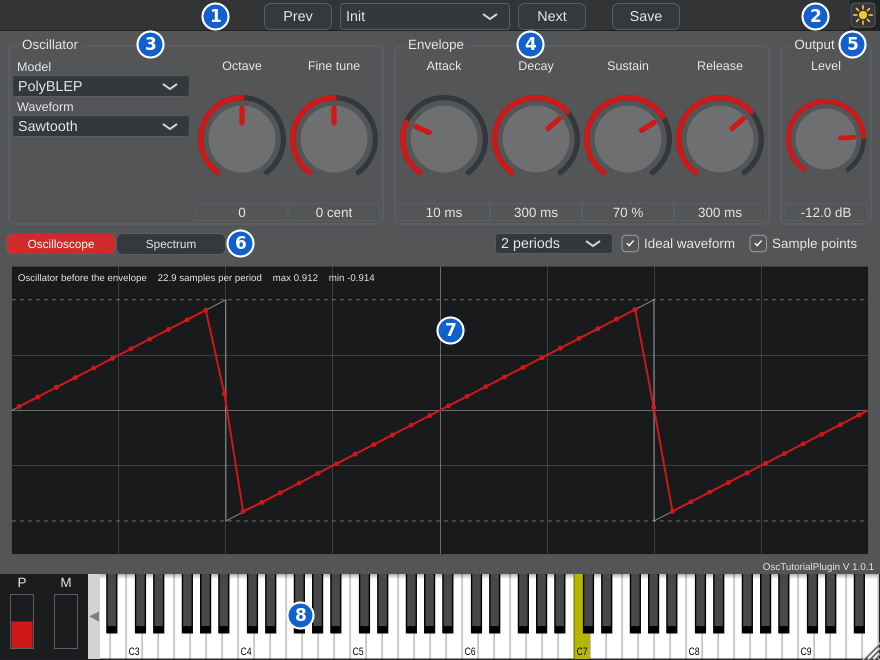
\includegraphics[width=0.9\textwidth]{images/GUI_Numbers.png}
\end{center}
\begin{enumerate}
    \item \textbf{Preset handler}: Prev/Next step through the presets. To save a new preset,
    type a name and press Save. Save turns red when you change a parameter of the displayed
    preset; press it to update the preset. To delete a preset, delete its XML file.
    The preset \textbf{Init} always holds the default values; it is written again at every start,
    so save your own sounds under another name.
    \item \textbf{Day/night}: switches between the night (dark) and the day (light) theme.
    \item \textbf{Oscillator}: \emph{Model} (the method, section~\ref{sec:tutorial}), \emph{Waveform},
    \emph{Octave} ($-3$ \dots\ $+3$) and \emph{Fine tune} ($\pm 100$ cent).
    \item \textbf{Envelope}: a linear ADSR (attack, decay, sustain level, release).
    \item \textbf{Output}: the level (at velocity 127).
    \item \textbf{Page buttons}: switch the big view between the oscilloscope and the spectrum.
    \item \textbf{The big view.} \emph{Oscilloscope}: 1 or 2 periods of the oscillator \emph{before} the
    envelope (so the amplitude is always 1), started at the beginning of a period (phase 0), so the
    picture stands still. The thin line is the ideal waveform, the dots are the samples (shown when
    they are at least 4 pixels apart, i.e.\ for high notes). The top line shows the samples per
    period and the largest and smallest value. \emph{Spectrum}: FFT of the oscillator (8192 points,
    Blackman-Harris window), 0\,dB = a sine with amplitude 1, \emph{linear} frequency axis up to
    $f_s/2$. The thin vertical lines mark the harmonics of the fundamental: every peak between
    them is aliasing. The top line shows the energy outside the harmonics (section~\ref{sec:measure}).
    \item \textbf{Keyboard} with pitch wheel (P, $\pm 2$ semitones) and modulation wheel (M, not used).
    The synth is monophonic: the last key pressed sounds; releasing it brings back the previous key
    that is still held.
\end{enumerate}

\section{Controls}\label{sec:controls}
All controls, their range and default value. Rest the mouse on a control to see its
description as a tooltip.

\begin{center}
\small
% generated from the code: OscTutorialPlugin_Tester --manual tex > controls.tex (see docs/HowToDoc.md)
\begin{tabular}{p{0.2\textwidth}p{0.22\textwidth}p{0.12\textwidth}p{0.36\textwidth}}
\hline
Control & Range & Default & Description \\
\hline
Model & Naive - Oversampling 8x & Naive & How the oscillator makes the waveform: Naive (sampled ideal waveform, aliasing), Wavetable (band-limited tables, one per octave), PolyBLEP and PolyBLEP 4-point (naive waveform with polynomial corrections at jumps and corners), minBLEP (minimum-phase corrections from a table), BLIT (integrated band-limited impulse trains), DPW (differentiated antiderivative), Oversampling 8x (naive at 8 fs, filtered). \\
Waveform & Sine - Sawtooth & Sawtooth & The waveform of the oscillator (Rectangle: 50 \% duty cycle). \\
Lanczos sigma & Off - On & Off & Wavetable only: weights the harmonics with Lanczos sigma factors, which reduces the overshoot at jumps (Gibbs phenomenon) from 9 \% to about 1 \%. \\
Octave & -3 - 3 & 0 & Shifts the pitch by whole octaves. \\
Fine tune & -100 cent - 100 cent & 0 cent & Fine tuning in cent (100 cent = 1 semitone). \\
Attack & 1 ms - 5000 ms & 10 ms & Time to rise to full level after a key is pressed. \\
Decay & 1 ms - 5000 ms & 300 ms & Time to fall from full level to the sustain level. \\
Sustain & 0 \% - 100 \% & 70 \% & Level while the key is held (in \% of full level). \\
Release & 1 ms - 5000 ms & 300 ms & Time to fall to silence after the key is released. \\
Level & -60.0 dB - 0.0 dB & -12.0 dB & Output level (at velocity 127). \\
\hline
\end{tabular}

\end{center}

\section{Tutorial: the oscillator models}\label{sec:tutorial}

\subsection{Why the naive oscillator aliases}
A digital oscillator keeps a \emph{phase} $p \in [0, 1)$ and adds $\Delta p = f_0 / f_s$ at every
sample ($f_0$: frequency of the note, $f_s$: sample rate). The simplest idea is to compute the ideal
waveform at this phase: the sawtooth is $2p - 1$, the rectangle is $\pm 1$.

The ideal sawtooth has a jump in every period, and a jump has infinitely many harmonics:
\[
  s(t) = \frac{2}{\pi} \sum_{k=1}^{\infty} \frac{(-1)^{k+1}}{k} \sin(2\pi k f_0 t).
\]
Sampling cannot represent frequencies above $f_s/2$. A harmonic at $k f_0 > f_s/2$ is not lost, it
\emph{folds back} (aliases) to
\[
  f_\text{alias} = \left| k f_0 - m f_s \right| \quad \text{(the integer } m \text{ that brings it below } f_s/2\text{)}.
\]
These aliases are not harmonics of $f_0$: they sound inharmonic, rough, like a ring modulator, and they
even move in the opposite direction when you bend the pitch up. Their level falls only like $1/k$
(sawtooth, rectangle) or $1/k^2$ (triangle; it has corners, no jumps). So: the higher the note,
the more harmonics lie above $f_s/2$, and the worse it gets. The sine has only one harmonic and
never aliases (below $f_s/2$).

Every method below answers the same question differently: \emph{how do we get the harmonics below
$f_s/2$ without the ones above?}

\subsection{Naive}
\textbf{Idea:} the ideal waveform, evaluated at the phase of each sample.
\modelfigures{naive}{Naive}
The oscilloscope shows the perfect shape -- the jump falls exactly between two samples. That is the
trap: the samples look right, but the spectrum is full of aliases (the dense lines between the
harmonic marks; about $-13$\,dB of the energy are aliases).

\textbf{Pros:} trivial, cheap, exact shape, no delay.
\textbf{Cons:} strong aliasing for all waveforms with jumps or corners, getting worse with pitch.
Acceptable only for low notes or for LFOs.

\subsection{Wavetable}
\textbf{Idea:} store one period of the waveform in a table, computed by additive synthesis with only
the harmonics that fit below $f_s/2$. One table per octave of the fundamental (10 tables of 2048
samples per waveform; table $k$ is used for fundamentals up to $40\,\text{Hz} \cdot 2^k$ and has all
harmonics below $f_s/2$ for its highest note). Read with linear interpolation.
\modelfigures{wavetable}{Wavetable}
The spectrum is clean ($-86$\,dB). The oscilloscope shows the price of a band-limited jump: it
overshoots and rings (Gibbs phenomenon, see section~\ref{sec:gibbs}). Note also that the spectrum ends
at the 9th harmonic (18.8\,kHz): at C7 the table for fundamentals up to 2560\,Hz is used, and it can only
have 9 harmonics. Notes in the lower part of an octave lose up to one octave of bandwidth.

\textbf{Pros:} the cheapest method of all when running (one table lookup and one interpolation),
almost no aliasing, works for any waveform you can describe by its harmonics.
\textbf{Cons:} memory (here 330\,kB per model), tables must be built (here at \texttt{prepareToPlay}),
brightness steps at the table boundaries (could be avoided by crossfading two tables), interpolation
errors, and the waveform is fixed (no hard sync, no pulse-width modulation without extra tables).

\subsection{Wavetable + Lanczos}
The same tables, but harmonic $k$ is weighted with the Lanczos sigma factor (section~\ref{sec:gibbs}).
\modelfigures{lanczos}{Wavetable + Lanczos}
The overshoot is gone, the top harmonics are a little weaker (compare the spectra).

\textbf{Pros:} no ringing, otherwise as Wavetable.
\textbf{Cons:} slightly duller, especially at high notes (few harmonics, so the sigma factors fall early).

\subsection{PolyBLEP (2-point)}
\textbf{Idea:} keep the naive waveform but repair each jump. A band-limited step (BLEP) differs from the
ideal step only near the jump. PolyBLEP approximates this difference by a short polynomial and adds it to
the samples around the jump. With $d$ = distance to the jump in samples and a jump of height 1:
\[
  r(d) = \begin{cases} \tfrac12 (1 + d)^2 & -1 < d \le 0 \text{ (before)}\\
  -\tfrac12 (1 - d)^2 & 0 < d < 1 \text{ (after)} \end{cases}
\]
This is the integral of a triangular pulse of 2 samples width minus the ideal step. Corners (triangle)
get its integral, the polyBLAMP $(1 - |d|)^3/6$ per change of the slope. Because the phase tells us where
the next jump is, the correction can also be applied \emph{before} the jump.
\modelfigures{polyblep}{PolyBLEP}
The dots show it: only the two samples next to each jump are changed. The spectrum is much better than
naive ($-29$\,dB), but the aliases near $f_s/2$ remain (the residual is short, so it is not a good low-pass).

\textbf{Pros:} cheap, no tables, no delay, works with changing frequency and with tricks like hard sync and
pulse-width modulation (a jump can be anywhere), easy to understand.
\textbf{Cons:} only moderate suppression; damps the top octave a bit.

\subsection{PolyBLEP 4-point}
The same with a smoother band-limited impulse: a cubic B-spline over 4 samples. The residual is a
piecewise polynomial of degree 4 (degree 5 for the BLAMP), see \texttt{PolyBlepOscillator.cpp}.
\modelfigures{polyblep4}{PolyBLEP 4-point}
About 10\,dB better than the 2-point version ($-38$\,dB), at almost the same cost. The B-spline is also
a stronger low-pass: the harmonics near $f_s/2$ are weaker.

\subsection{minBLEP}
\textbf{Idea:} use a \emph{long, good} band-limited step instead of a short polynomial: a windowed sinc
(16 zero crossings on each side) integrated to a step. A symmetric step would need 16 samples of the
future. The trick (Brandt 2001): make it \emph{minimum phase} (via the real cepstrum), so all of its
correction lies \emph{after} the jump, and store it in a table (64 points per sample). At every jump
the table is added to the next 32 samples.
\modelfigures{minblep}{minBLEP}
The spectrum is as clean as the wavetable ($-85$\,dB). The oscilloscope looks different: no ringing
before the jump, more after it, and the whole waveform is \textbf{delayed} by about 3 samples. Next to the
ideal curve, the rising ramp therefore lies \emph{below} it -- this is not an offset (the mean is 0), it is
the delay: a ramp that comes 3 samples later is lower at the same moment.

\textbf{Pros:} excellent suppression, works for jumps anywhere (hard sync, PWM).
\textbf{Cons:} more complex (table, ring buffer of corrections), delay and changed phase of the harmonics,
asymmetric overshoot (here up to 1.44 for the rectangle). Found while building it: with the cut-off of the
sinc exactly at $f_s/2$, the transition band of the window lies half above $f_s/2$ and aliases; the cut-off is
therefore $0.85\,f_s/2$.

\subsection{BLIT}
\textbf{Idea} (Stilson \& Smith 1996): start from the derivative. The derivative of a sawtooth is a constant
minus an impulse train; the derivative of a rectangle is a train of alternating impulses. A
\emph{band-limited} impulse train (BLIT) can be computed in closed form (Dirichlet kernel with
$M = 2\lfloor P/2 \rfloor + 1$ terms, $P$ = period in samples):
\[
  \text{blit}(x) = \frac{1}{P}\, \frac{\sin(\pi M x)}{\sin(\pi x)}.
\]
Integrating it gives band-limited waveforms. The integrators must be \emph{leaky} (slightly below 1),
otherwise numerical errors accumulate.
\modelfigures{blit}{BLIT}
Very clean ($-83$\,dB). But the oscilloscope shows three side effects, all worth discussing:
(1) the overshoot is larger than the Gibbs value (1.2 \dots\ 1.3): the running sum $y_n = y_{n-1} + x_n$ is not a
true integrator, it boosts the harmonics near $f_s/2$ by up to $\pi/2$; (2) there is ringing near $f_s/2$
all over the period (the Dirichlet kernel decays slowly); (3) the leak (1\,Hz) tilts the flat parts of
the rectangle at low notes:
\begin{center}
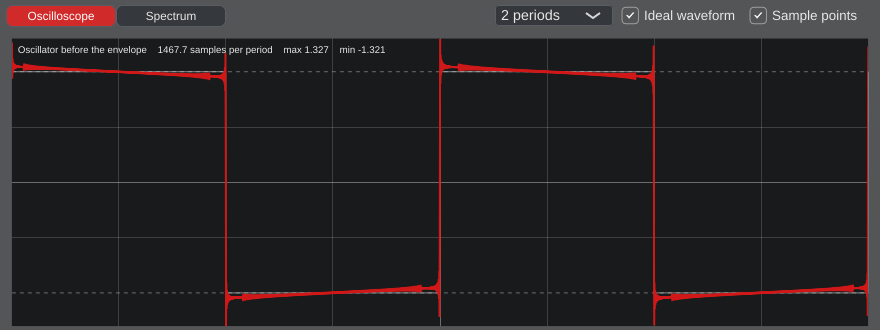
\includegraphics[width=0.6\textwidth]{images/blit_low.png}\\[-1ex]
{\small BLIT rectangle at C1 (32.7\,Hz): the tilt of the leaky integrator and the ringing next to the jumps.}
\end{center}
The triangle is a second integration of a rectangle. Two integrators in series amplify every small DC error
enormously, so the triangle path needs a stronger leak (5\,Hz).

\textbf{Pros:} elegant theory, full bandwidth up to $f_s/2$, no tables.
\textbf{Cons:} the most expensive of the analytic methods (several $\sin$ per sample), leaky integrators
(tilt, start transients, DC), not easy for jumps at arbitrary times.

\subsection{DPW (differentiated parabolic waveform)}
\textbf{Idea} (Välimäki 2005): compute the \emph{antiderivative} $F$ of the waveform instead of the waveform
itself and differentiate numerically:
\[
  y_n = \frac{F(p_n + \Delta p/2) - F(p_n - \Delta p/2)}{\Delta p}.
\]
For the sawtooth $F = s^2/4$, a parabola -- hence the name. This is the mean of the naive waveform over
one sample interval: a box filter, so the harmonics fall like $1/k^2$ instead of $1/k$ before they are
sampled.
\modelfigures{dpw}{DPW}
The jumps become ramps of one sample. About 10\,dB better than naive ($-23$\,dB).

\textbf{Pros:} extremely simple, cheap, no delay (centred difference), no tables, works for every
waveform whose antiderivative you know. Higher orders (DPW3, DPW4: higher antiderivatives, repeated
differences) are much better.
\textbf{Cons:} first order is only a weak improvement; the difference of two large numbers loses
precision at low notes (we use \texttt{double}).

\subsection{Oversampling 8x}
\textbf{Idea:} the brute-force method: run the naive oscillator at $8 f_s$, low-pass filter (FIR, 512 taps,
windowed sinc, cut-off $0.42 f_s$) and keep every 8th sample. Only harmonics above $4 f_s$ still fold back
into the audio band, and they are weak.
\modelfigures{oversampling}{Oversampling 8x}
About $20 \log_{10} 8 = 18$\,dB better than naive for the jumps ($-32$\,dB); for the triangle (harmonics with
$1/k^2$) much more ($-80$\,dB). The filter rings like the wavetable (it is a band limit, too).

\textbf{Pros:} easy to understand, works for \emph{everything}, also for non-linear processes (distortion,
waveshaping, FM) where the other tricks fail. The general tool.
\textbf{Cons:} by far the most expensive (8 naive samples and 512 multiplications per output sample), and
for jumps still not very good; the filter delays (here compensated by running the oscillator ahead).

\subsection{Comparison}\label{sec:measure}
\textbf{Aliasing} = energy outside the harmonics (and DC), relative to the total energy, in dB; the same
number as on the spectrum page. Measured with \texttt{tools/analysis/measure\_models.py} (1\,s, Blackman
window, 48\,kHz). The floor of this measurement is about $-57$\,dB at C4 and $-93$\,dB at C7.
\textbf{Cost} = computing time per sample (sawtooth, C7), measured on a desktop PC (Linux, gcc -O2);
for comparison: 1\,\% of one core at 48\,kHz is 208\,ns per sample.

\begin{center}
\small
\begin{tabular}{lrrrrrr}
\toprule
 & \multicolumn{3}{c}{sawtooth aliasing [dB]} & rectangle & triangle & cost \\
Model & C4 & C7 & C8 & max (C7) & C7 [dB] & [ns/sample] \\
\midrule
Naive               & $-21.8$ & $-12.8$ & $-9.6$  & 1.00 & $-40.3$ & 5.6 \\
Wavetable           & floor   & $-85.5$ & $-82.7$ & 1.18 & $-92.5$ & 3.7 \\
Wavetable + Lanczos & floor   & $-88.4$ & $-84.9$ & 1.02 & $-92.8$ & 3.7 \\
PolyBLEP            & $-37.7$ & $-28.5$ & $-23.8$ & 1.00 & $-54.0$ & 11.6 \\
PolyBLEP 4-point    & $-47.3$ & $-38.4$ & $-32.9$ & 1.00 & $-65.0$ & 13.5 \\
minBLEP             & floor   & $-85.3$ & $-82.2$ & 1.44 & $-92.5$ & 19.4 \\
BLIT                & floor   & $-83.0$ & $-79.9$ & 1.30 & $-92.2$ & 110 \\
DPW                 & $-31.9$ & $-22.6$ & $-18.5$ & 1.00 & $-48.0$ & 20.0 \\
Oversampling 8x     & $-41.5$ & $-32.2$ & $-28.8$ & 1.19 & $-80.2$ & 396 \\
\bottomrule
\end{tabular}
\end{center}

\textbf{Rules of thumb.}
Fixed waveforms and lowest cost: \emph{wavetable} (with Lanczos if the ringing matters).
Jumps at arbitrary moments (hard sync, PWM, changing shapes), no tables: \emph{polyBLEP} (4-point if you can
afford it), or \emph{minBLEP} if quality matters and a few samples of delay do not.
Anything non-linear: \emph{oversampling}.
\emph{Naive} only for LFOs and low notes; \emph{BLIT} and \emph{DPW} mainly for understanding (and DPW of higher
order as a cheap alternative to polyBLEP).

\subsection{The Gibbs phenomenon and Lanczos sigma factors}\label{sec:gibbs}
A Fourier series that is cut off after $H$ harmonics overshoots at every jump by about 9\,\% of the jump
(for a rectangle from $-1$ to $+1$: up to 1.18), \emph{however large $H$ is}. More harmonics only make the
ringing narrower, not lower. Every band-limited jump rings like this -- the wavetable, the oversampling
filter, minBLEP and BLIT all show it.

Lanczos (1956) proposed to weight harmonic $k$ with
\[
  \sigma_k = \operatorname{sinc}\!\left(\frac{k}{H+1}\right) = \frac{\sin\left(\pi k/(H+1)\right)}{\pi k/(H+1)}.
\]
This is the same as averaging the cut-off series over one period of its highest harmonic: the ringing is
smoothed away, the overshoot falls to about 1\,\%. The price is a gentle low-pass on the top octave. A sine
is not a cut-off series and gets no sigma factor.
\begin{center}
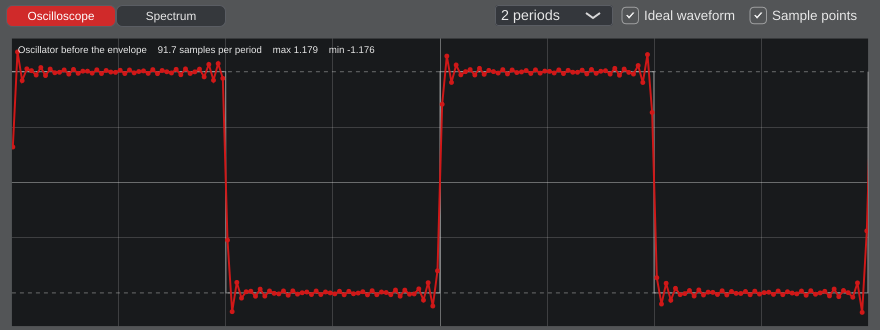
\includegraphics[width=0.49\textwidth]{images/gibbs_wavetable.png}\hfill
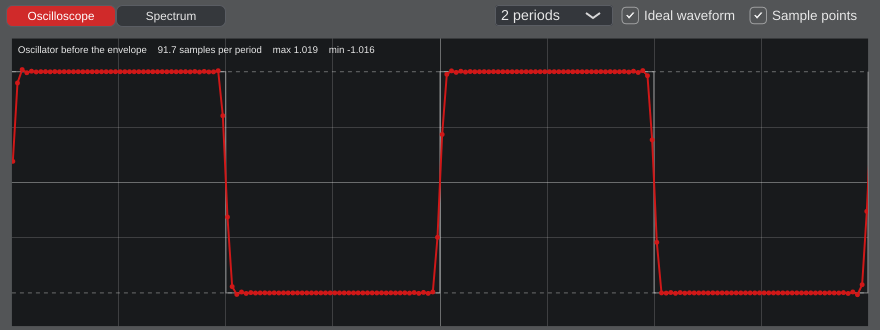
\includegraphics[width=0.49\textwidth]{images/gibbs_lanczos.png}\\[-1ex]
{\small Rectangle at C5 (37 harmonics). Left: Wavetable, max 1.18. Right: Wavetable + Lanczos, max 1.02.}
\end{center}
Try it with the presets \emph{Gibbs Demo} and \emph{Lanczos Demo}.

\section{Exercises}\label{sec:exercises}
\begin{enumerate}
\item \textbf{Hear aliasing.} Load \emph{Aliasing Demo} (naive rectangle, two octaves up) and play a slow
  scale upwards. Describe what you hear. Bend the pitch with the wheel: in which direction do the
  aliases move?
\item \textbf{Predict an alias.} Naive sawtooth at C7 ($f_0 = 2093$\,Hz), $f_s = 48$\,kHz. Where does the
  12th harmonic appear? (Answer: $12 f_0 = 25116$\,Hz $\to$ $48000 - 25116 = 22884$\,Hz.) Find it on the
  spectrum page.
\item \textbf{Compare the models.} On the spectrum page, play C7 with the sawtooth and step through all
  models. Note the value ``outside the harmonics'' and compare with the table above. Repeat with the
  triangle: why is the naive triangle so much better than the naive sawtooth?
\item \textbf{Where does the correction act?} Oscilloscope, PolyBLEP, C7: which samples differ from the
  ideal waveform? Now PolyBLEP 4-point and minBLEP.
\item \textbf{Gibbs.} Wavetable, rectangle: play C3, C5 and C7. What happens to the width and to the height
  of the ringing? Then Wavetable + Lanczos.
\item \textbf{Minimum phase.} minBLEP, sawtooth, C6: estimate the delay against the ideal curve. Why can
  a minimum-phase step not ring \emph{before} the jump?
\item \textbf{BLIT.} BLIT, rectangle, C1 (Octave $-1$): explain the tilt. What would happen without the
  leak?
\item \textbf{Cost.} Which model would you choose for a 64-voice polyphonic synth on a small embedded
  processor? Which one for a distortion effect? Give reasons.
\item \textbf{Code.} Read \texttt{oscillators/PolyBlepOscillator.cpp} and derive the 2-point polyBLEP
  residual yourself (integrate a triangular pulse, subtract the step).
\end{enumerate}

\section{How it works}
\begin{verbatim}
MIDI (DAW or on-screen keyboard)
  -> note stack (monophonic, last note), pitch bend, velocity
  -> oscillator (one of 9 models)  --> oscilloscope / spectrum
  -> linear ADSR envelope  -> level  -> both output channels
\end{verbatim}
The frequency is $f = 440\,\text{Hz} \cdot 2^{(n - 69 + 12\,\text{octave} + \text{cent}/100 + \text{bend})/12}$
($n$: MIDI note), limited to $0.45 f_s$. Parameters are read every 2\,ms (synchronous blocks); notes
start at the exact sample of the MIDI event. The internal block processing delays the output by 2\,ms;
the plug-in reports this latency to the host. All models are phase aligned (all waveforms start at 0
and rise), so the model can be switched while a note sounds; the new model continues at the phase of
the old one.

\section{Source code}
OscTutorialPlugin is open source. You find the source code here:\newline
\url{\sourceurl}. Please report bugs there, too. Start reading with \texttt{oscillators/Oscillator.h};
each model has its own file. \texttt{planning.md} documents the decisions, the measurements and ideas
how to go on.

\section{References}
\begin{itemize}
\item T.~Stilson, J.~Smith: Alias-free digital synthesis of classic analog waveforms. ICMC 1996 (BLIT).
\item E.~Brandt: Hard sync without aliasing. ICMC 2001 (minBLEP).
\item V.~Välimäki: Discrete-time synthesis of the sawtooth waveform with reduced aliasing. IEEE Signal
  Processing Letters 12(3), 2005 (DPW).
\item V.~Välimäki, A.~Huovilainen: Antialiasing oscillators in subtractive synthesis. IEEE Signal
  Processing Magazine 24(2), 2007 (polyBLEP).
\item V.~Välimäki, J.~Pekonen, J.~Nam: Perceptually informed synthesis of bandlimited classical waveforms
  using integrated polynomial interpolation. JASA 131(1), 2012 (higher-order polyBLEP).
\item F.~Esqueda, V.~Välimäki, S.~Bilbao: Rounding corners with BLAMP. DAFx 2016 (polyBLAMP).
\item C.~Lanczos: Applied Analysis. Prentice Hall, 1956 (sigma factors).
\end{itemize}

\section{Legal stuff}
For this documentation the CC-BY 4.0 licence is valid. Copyright holder is \pluginauthor.
The source code of the plug-in is under the MIT licence. The plug-in binaries contain JUCE
(used under the AGPLv3), the VST3 SDK (MIT) and, on macOS, the Audio Unit SDK (Apache 2.0);
the binaries as a whole are distributed under the AGPLv3.

\begin{itemize}
    \item Microsoft\textsuperscript{\textregistered}, Windows\textsuperscript{\textregistered}
    are trademarks of the Microsoft group of companies.
    \item Mac\textsuperscript{\textregistered} is a trademark of Apple Inc.
    \item VST\textsuperscript{\textregistered} is a registered trademark of Steinberg Media
    Technologies GmbH.
\end{itemize}

\end{document}
